\documentclass[11pt]{article}
\usepackage{lmodern,setspace,amsmath,amssymb,amsfonts,amsthm,graphicx,multicol,grffile,float}
\usepackage{authblk,url,csvsimple,cuted,dblfloatfix,parskip}
\usepackage[a4paper, top=0.9in, bottom=1.05in, left=0.65in, right=0.65in]{geometry}
\usepackage[polish]{babel}
\usepackage[utf8]{inputenc}
\usepackage[unicode]{hyperref}
\usepackage{listings}
\usepackage{booktabs}
\title{Informatyka w Medycynie - Projekt 2\\ Wykrywanie naczyń dna siatkówki oka}
\author{Dariusz Max Adamski 136674, Sławomir Gilewski 142192}
\affil{\{dariusz.adamski,slawomir.gilewski\}@student.put.poznan.pl}
\date{Data oddania: \today}

\def\code#1{\texttt{#1}}

\begin{document}

\maketitle

\section*{Wstęp}

W sprawozdaniu przedstawimy nasze rozwiązanie problemu wykrywania naczyń dna siatkówki oka.
Opiszemy i porównamy dwie metody. Pierwsza z nich korzysta z klasycznych technik przetwarzania obrazów,
natomiast druga z nadzorowanych metod uczenia maszynowego.

\section{Narzędzia}

\subsection{Język Programowania}
Wybraliśmy język programowania Python i środowisko Jupyter Notebook. Głównie ze względu na jego prostotę i łatwość instalowania i korzystania z dodatkowych bibliotek.

\subsection{Dodatkowe biblioteki}
Istotne biblioteki i ich wykorzystanie w naszym programie to:
\begin{itemize}
    \item Numpy: Obliczenia i operacje na n-wymiarowych macierzach
    \item Pandas: Operacje na tabelach danych
    \item Scikit-learn: Gotowe narzędzia uczenia maszynowego
    \item Imblearn: Procedury do niezbalansowanych danych
    \item OpenCV i Scikit-Image: Przetwarzanie obrazu
    \item Matplotlib: Wszelkiego rodzaju wizualizacje
\end{itemize}

\section{Przetwarzanie obrazów}
\subsection{poszczególne kroki przetwarzania obrazu}
1. Wybieramy kanał zielony z modelu RGB.

Zwizualizowaliśmy wszystkie 3 kanały RGB i okazało się, że kanał zielony pozwala zobaczyć najwięcej naczyń i zdecydowanie powinien ułatwić programowi znalezienie ich.

\begin{figure}[h]
    \centering
	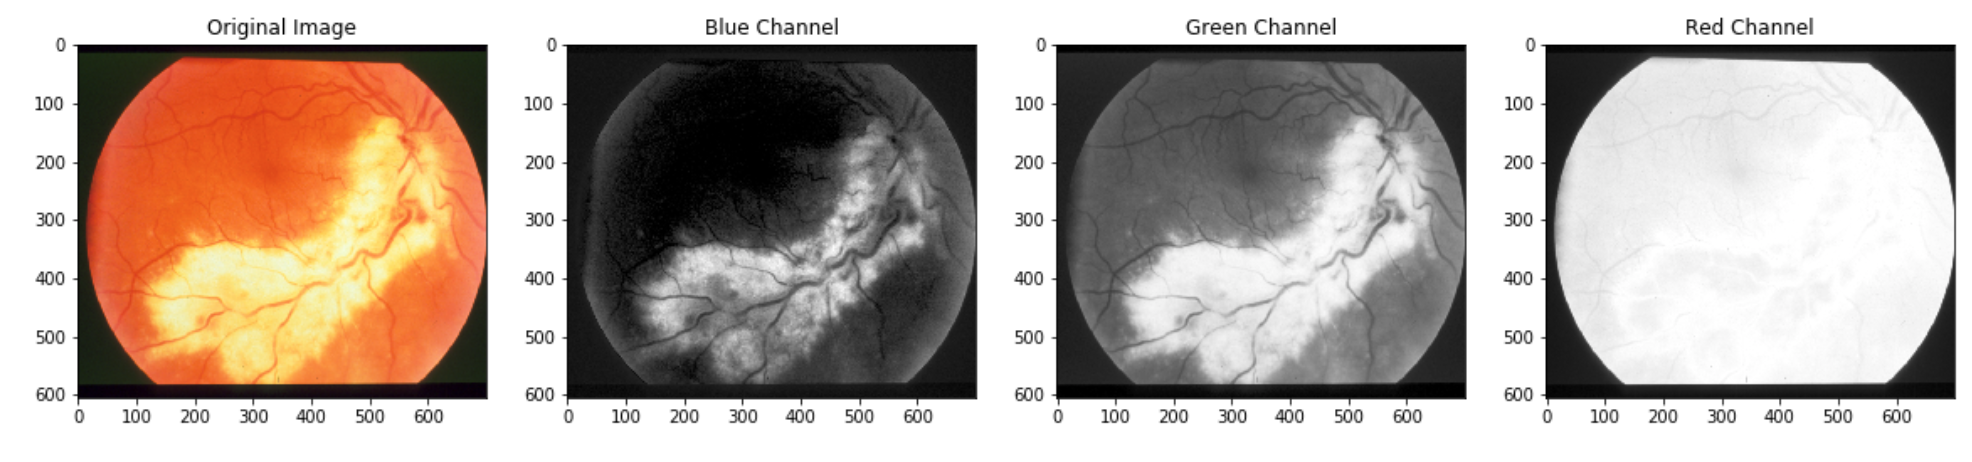
\includegraphics[scale=0.4]{res/img_pro_1.png}
	\caption{Kanały RGB obrazu}
	\label{fig:demo}
\end{figure}
\newpage
2. Wyrównujemy histogram (Histogram equalization).

Aby zwiększyć różnice pomiędzy różnymi odcieniami w obrazie, stosujemy "histogram equalization". Wybraliśmy metodę Contrast Limited Adaptive Histogram Equalization, ponieważ wydaje się najskuteczniejsza.

\begin{figure}[h]
    \centering
	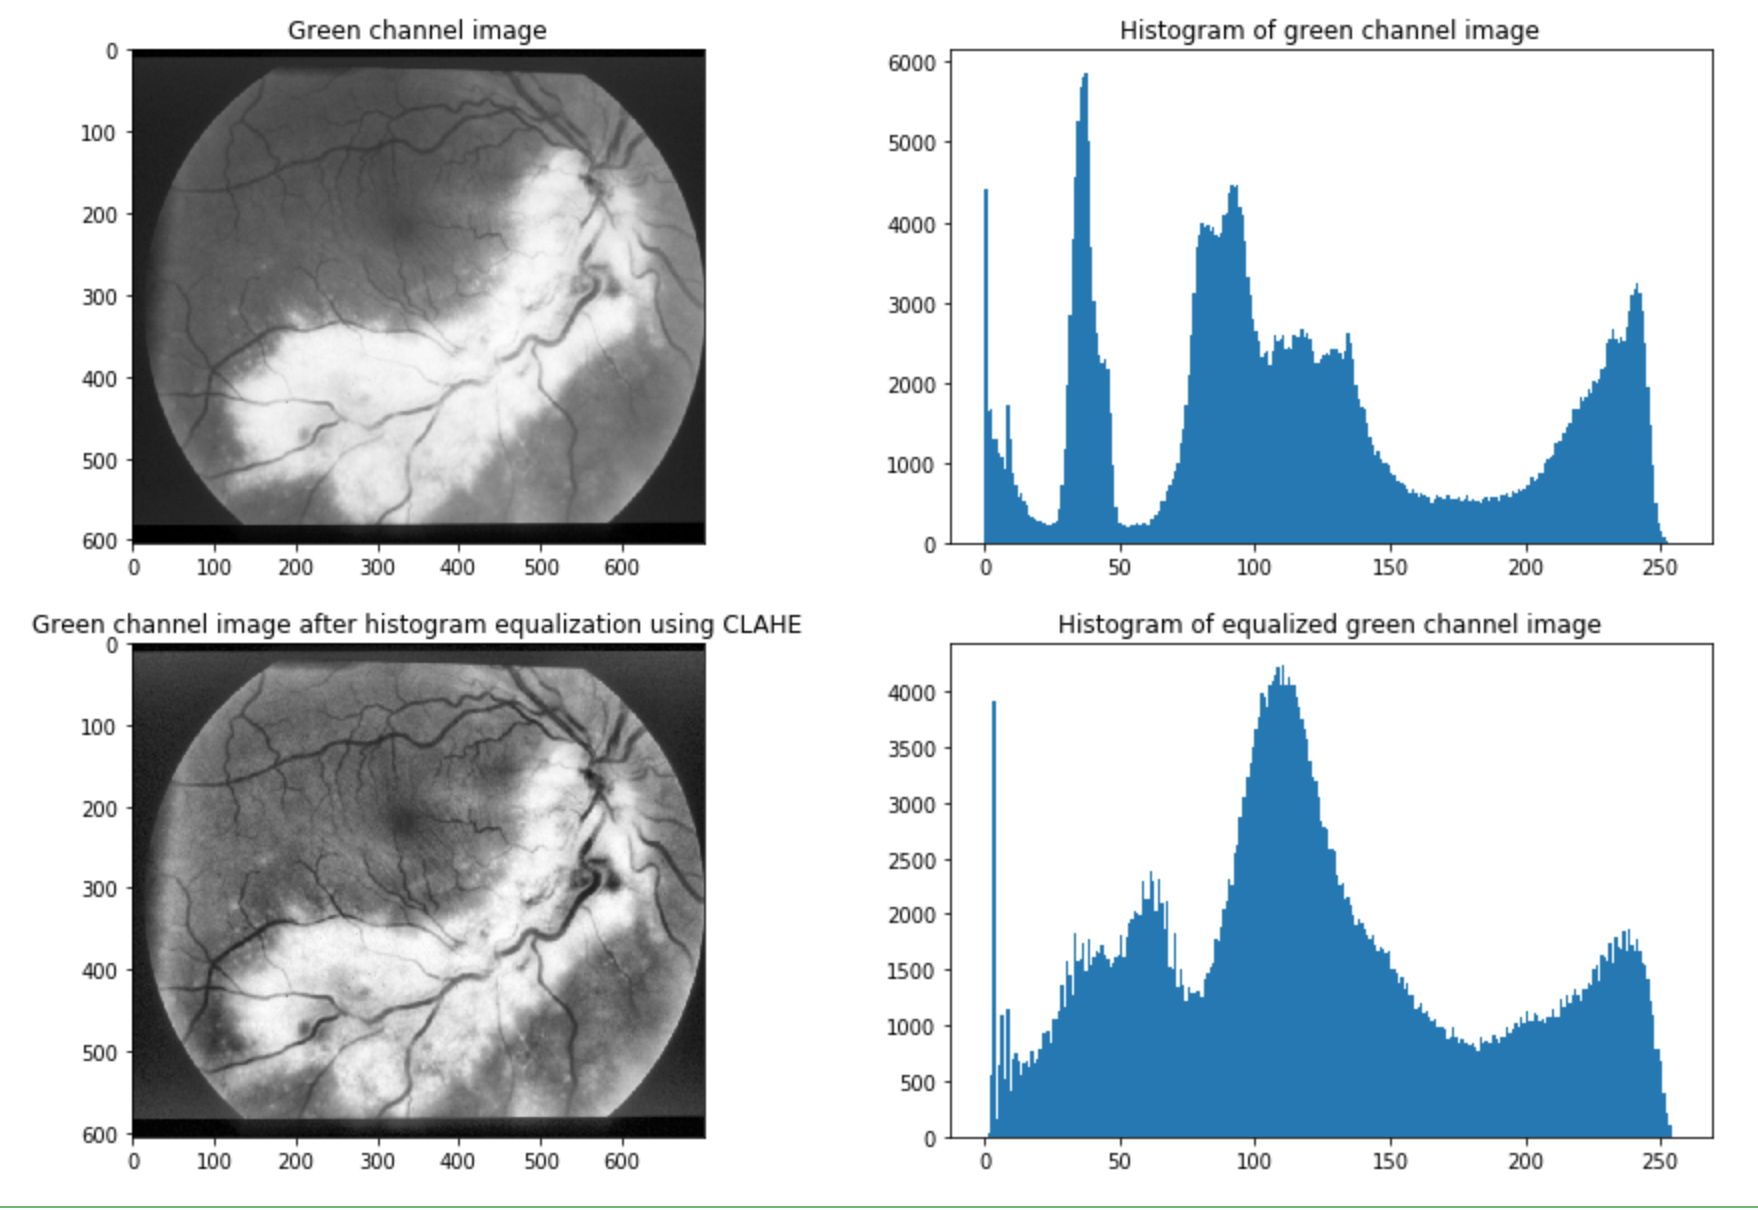
\includegraphics[scale=0.3]{res/img_pro_2.png}
	\caption{Wyrównanie histogramu}
	\label{fig:demo}
\end{figure}

3. Stosując operacje morfologiczne otwarcia i zamknięcia dokonujemy ekstrakcji tła naczyń krwionośnych. 

Stosując naprzemiennie operację otwarcia i zamknięcia oraz stosując różne wielkości jądra (kernel) wyciągamy z obrazka tło, na którym znajdują się nasze naczynia krwionośne.

\begin{figure}[h]
    \centering
	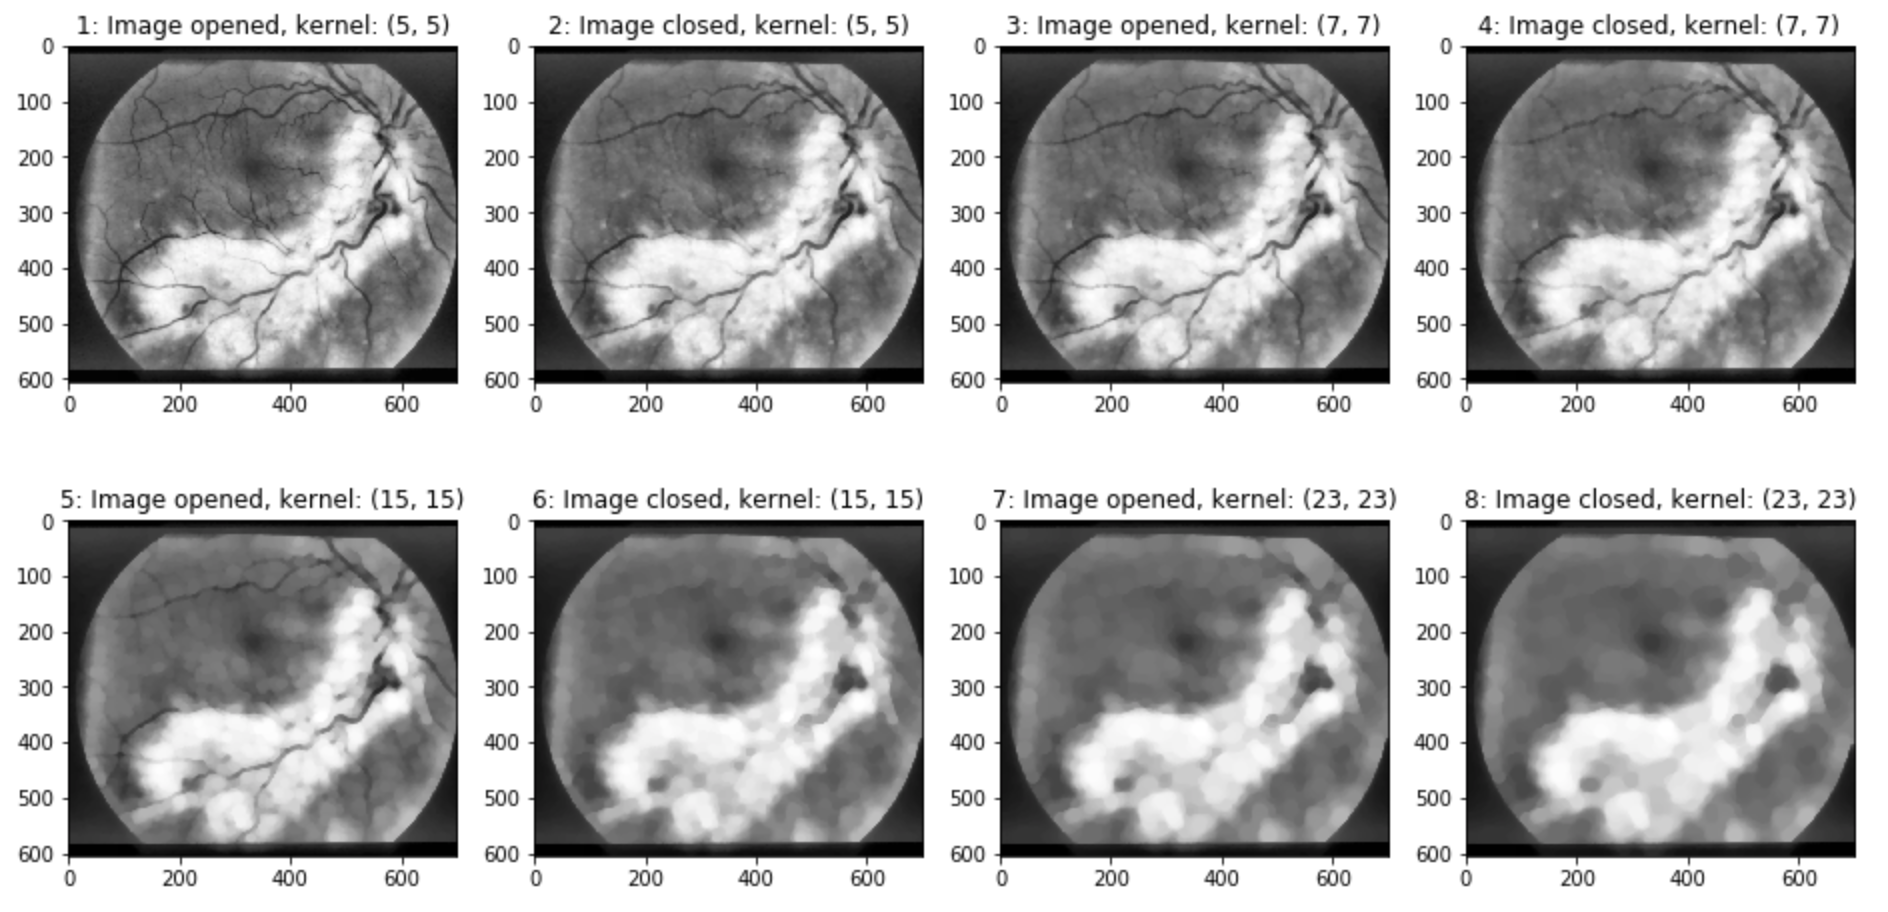
\includegraphics[scale=0.3]{res/img_pro_3.png}
	\caption{Operacje morfologiczne}
	\label{fig:demo}
\end{figure}
\newpage

4. Odejmujemy nasz obraz od otaczającego go tła.

Ponieważ naczynia krwionośne są ciemne (mniejsza wartość pixela), odejmujemy nasz obraz od tła. Dzięki temu powinny zostać nam jedynie naczynia. Technika ta pojawiła się w książce "Deserno, T. M. (2011). Biomedical image processing.\" w rozdziałach 4.2.2 oraz 4.3.2.

\begin{figure}[h]
    \centering
	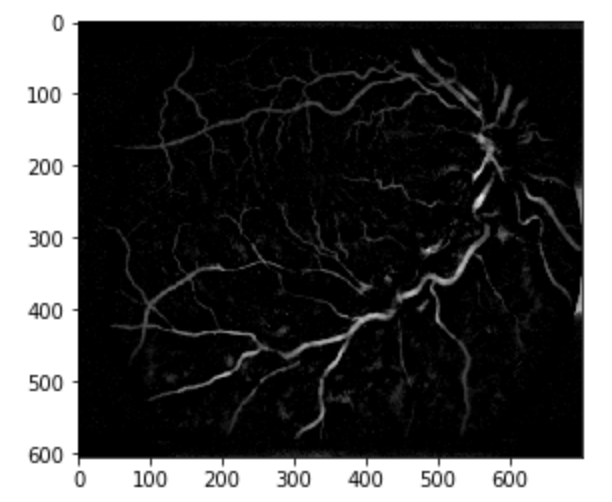
\includegraphics[scale=0.5]{res/img_pro_4.png}
	\caption{Wyekstrahowane naczynie}
	\label{fig:demo}
\end{figure}

5. Ponownie wyrównujemy histogram.

\begin{figure}[h]
    \centering
	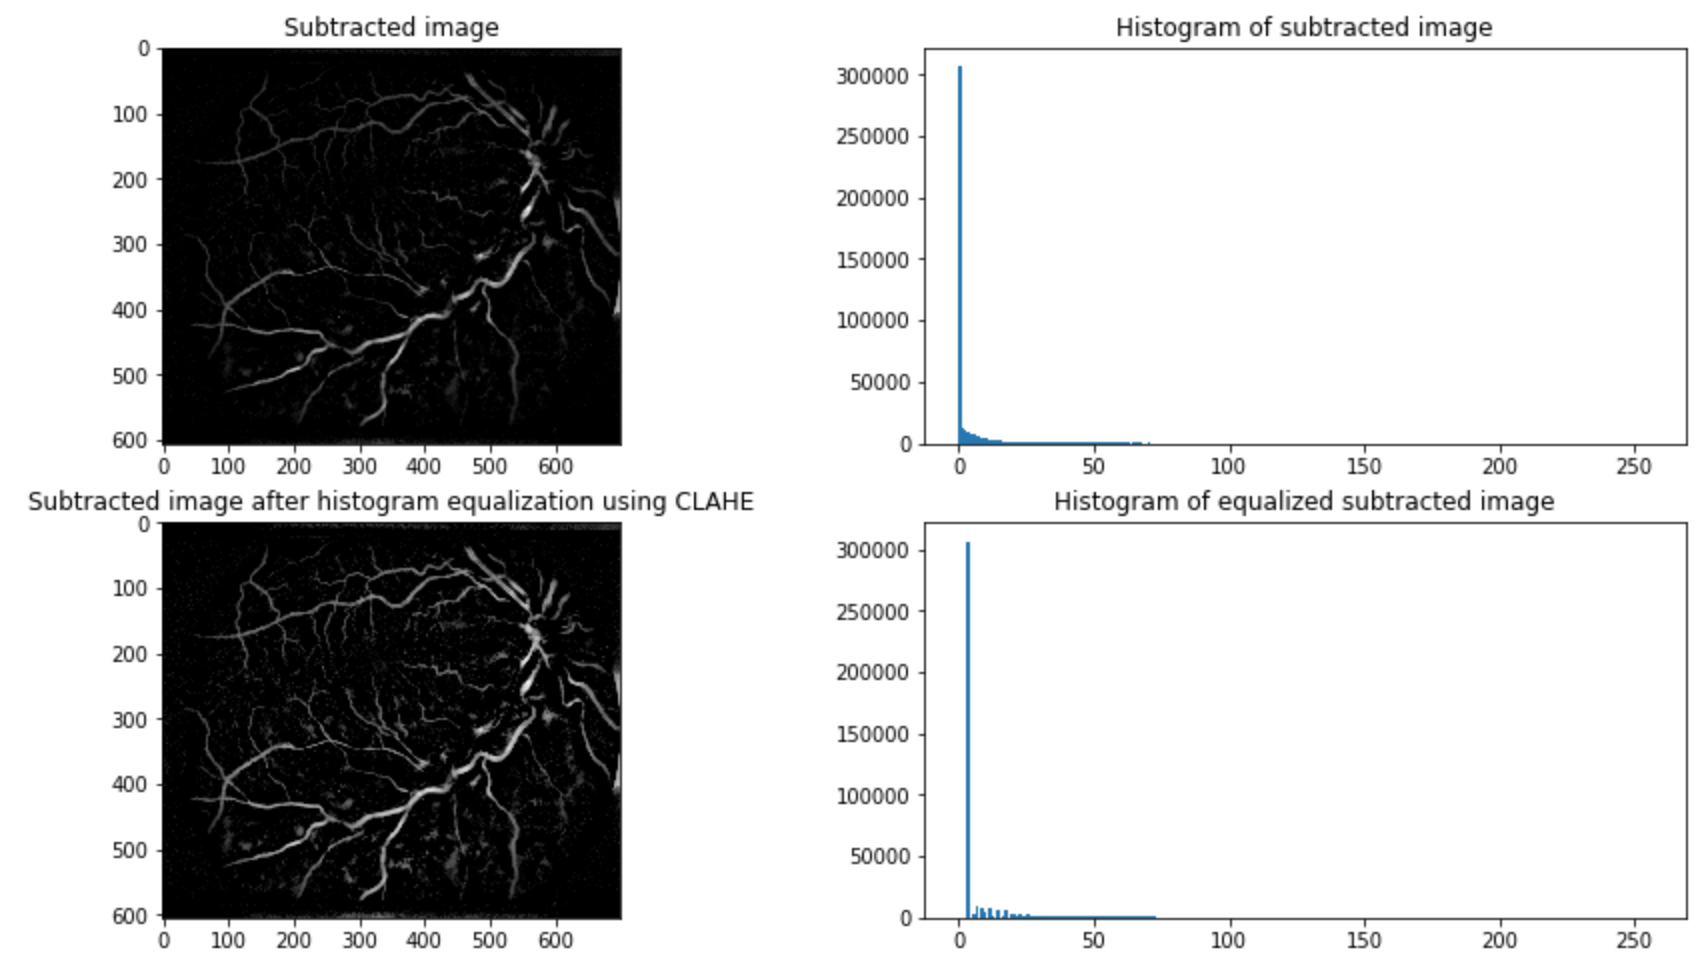
\includegraphics[scale=0.4]{res/img_pro_5.png}
	\caption{Wyrównanie histogramu}
	\label{fig:demo}
\end{figure}

6. Tworzymy maskę "zakłóceń".

Korzystając z biblioteki opencv oraz z faktu, że naczynia krwionośne są połączone w dłuższych "liniach", rysujemy na masce znalezione kontury, które mają wielkość mniejszą niż ustalona. 

\begin{figure}[h]
    \centering
	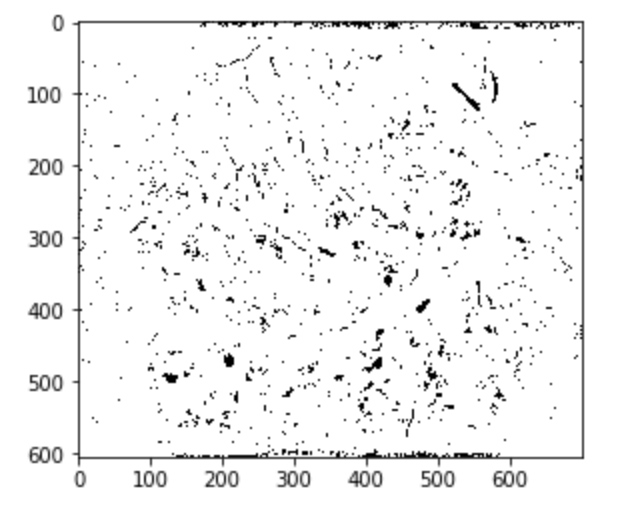
\includegraphics[scale=0.4]{res/img_pro_6.png}
	\caption{Maska zakłóceń}
	\label{fig:demo}
\end{figure}
\newpage
7. Filtrujemy obraz z naczyniami krwionośnymi.

Używając wcześniej utworzonej maski, wyciągamy jedynie te piksele z naszego obrazka, które przez maskę nie zostały uznane za szum.

\begin{figure}[h]
    \centering
	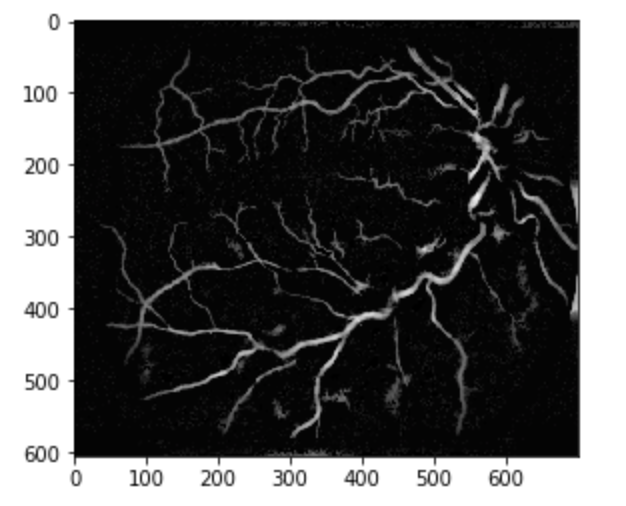
\includegraphics[scale=0.4]{res/img_pro_7.png}
	\caption{Przefiltrowany obraz}
	\label{fig:demo}
\end{figure}

8. Wykonujemy thresholding.

Za pomocą biblioteki opencv ekstrahujemy maskę naczyń krwionośnych korzystając z funkcji threshold.

\begin{figure}[h]
    \centering
	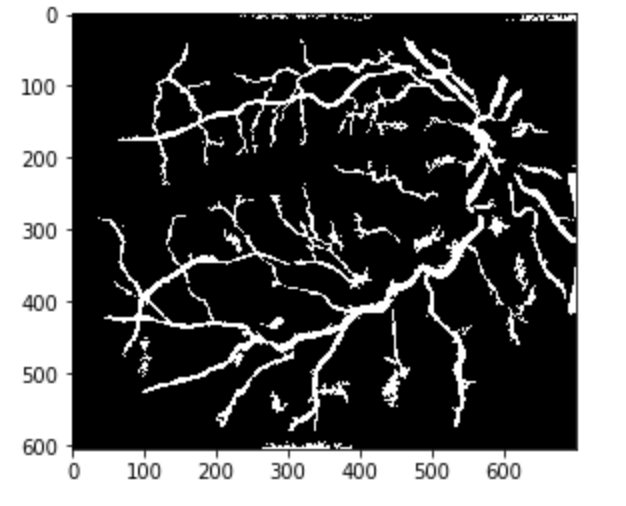
\includegraphics[scale=0.4]{res/img_pro_8.png}
	\caption{Wynik}
	\label{fig:demo}
\end{figure}

\subsection{krótkie uzasadnienie zastosowanego rozwiązania}

Takie rozwiązanie ma naszym zdaniem sens, ponieważ jest stosunkowo proste w idei oraz jest zaskakująco skuteczne jak na proste metody przetwarzania obrazu. Nie jest również zbyt wrażliwe na różne zakłócenia czy prześwietlenia obrazu, ponieważ niezależnie od nich, pozbywamy się problemu uzyskując obraz tła. Moglibyśmy je jeszcze ulepszyć o np szukanie naczyń krwionośnych podobną metodą na pozostałych kanałach rgb a następnie połączyć rozwiązania, jednak uznaliśmy, że nie jest to konieczne.

\section{Uczenie maszynowe}

\subsection{Przygotowanie danych}

Na początku podzieliliśmy zbiór danych na testowy (pierwsze 5 zdjęć) i treningowy (reszta zdjęć).
W sumie na zbiór testowy przypada około 13\% przykładów.
Podczas uczenia dzielimy zbiór treningowy, na właściwy treningowy i walidacyjny według 5-krotnej walidacji krzyżowej.

Zastosowaliśmy proste przetwarzanie wstępne obrazków.
Najpierw konwertujemy obrazek do przestrzeni kolorów \code{LAB} i
stosujemy łagodne filtrowanie bilateralne, w celu usunięcia szumu, przy zachowaniu krawędzi.
Następnie metodą \code{CLAHE} (clip limit = 2, grid size = 8) normalizujemy histogram kanału L.

Każdy obrazek i jego maskę dzielimy na wycinki o rozmiarze 5x5 przy pomocy funkcji \newline \code{skimage.view\_as\_windows}.
Jako etykietę wycinka przyjmujemy ,,1'' jeśli środkowy piksel wycinka maski jest biały, co oznacza, że jest naczyniem i ,,0'' w przeciwnym wypadku.

\subsection{Ekstrakcja cech}

Dla każdego wycinka wyznaczamy wektor cech dla klasyfikatora: średnią wartość i odchylenie standardowe każdego z kanałów \code{RGB} ($2 \times 3$ cechy), momenty centralne (10 cech), momenty obrotowe (7 cech) i momenty Hu (7 cech). W sumie wektor zawiera 40 cech. Cechy przykładów standaryzujemy przy pomocy \code{StandardScaler}, tak aby każda z nich miała średnią równą zero i wariancję równą jeden (średnią i wariancję liczymy tylko na przykładach ze zbioru treningowego). Robimy to aby algorytm nie priorytetyzował cech na podstawie średniej i wariancji. Pomimo tego, że standaryzacja nie jest wymagana dla ostatecznie wybranego przez nas algorytmu Random Forest, nie pominęliśmy tego kroku, żeby łatwiej móc testować inne algorytmy, które tego wymagały.

\subsection{Balansowanie danych}

Ponieważ w zbiorze uczącym występuje duża dysproporcja klas,
zastosowaliśmy technikę losowego undersamplingu.
Wykorzystaliśmy do tego gotową implementację z biblioteki \code{imblearn}.
Po balansowaniu proporcja klas pozytywnych do negatywnych w zbiorze treningowym wynosiła 1.

\subsection{Algorytm uczący}

Do klasyfikacji zastosowaliśmy algorytm Random Forest,
między innymi z uwagi na małe wymagania obliczeniowe,
pomimo zadowalających wyników w rożnych zadaniach klasyfikacji i regresji.

Liczbę drzew ustawiliśmy na \code{n\_estimators = 500}, głównie z powodu naszych ograniczeń sprzętowych.
Warto wspomnieć, że zwiększenie tego parametru zazwyczaj korzystnie wpływa na jakość modelu,
między innymi zmniejszając ewentualne przeuczenie.

Jako maksymalną liczbę cech rozważanych przez jedno drzewo przyjmujemy pierwiastek z całkowitej liczby cech.
Takie ustawienie jest często zalecane do klasyfikacji,
aby pozwolić drzewom ,,stać się ekspertami'' w wąskiej dziedzinie cech.

Innym ważnym parametrem jest maksymalna głębokość drzewa, którą ustawiliśmy na \code{max\_depth = 15}.
Domyślne ustawienie w Scikit-learn pozwala drzewom rosnąć bez ograniczeń,
co powoduje nadmierne dopasowanie do danych uczących (overfitting).

Dodatkowo ustawiliśmy parametry \code{min\_samples\_leaf = 0.005} i \code{min\_samples\_split = 0.03}.
Resztę parametrów zostawiliśmy domyślnych.

\subsection{Ocena modelu}

Wartości wszystkich parametrów (poza liczbą drzew i cech) wyznaczyliśmy wykonując
losowe przeszukiwanie przestrzeni parametrów z 5-krotną walidacją krzyżową.
Na końcu wybraliśmy model, który uzyskał najlepszą średnią wartość miary F1,
czyli harmonicznej średniej precyzji (precision) i czułości (recall),
na wszystkich foldach.
Wartość miary F1 na kolejnych foldach w zbiorze walidacyjnym wynosi: 0.8692, 0.8642, 0.8708, 0.8061, 0.6741.
Średnia wartość F1 wynosi: 0.8169, a jej odchylenie standardowe 0.0753.
Różnice interpretujemy jako zróżnicowanie zbioru danych, którego niestety nie możemy uniknąć.


\section{Wyniki}

\subsection{Wstęp}

Powierzchownie, porównując wyniki uzyskane metodami przetwarzania obrazu z wynikami uczenia maszynowego stwierdzamy,
że ręczne stworzenie filtrów i potoku przetwarzania obrazu zadziałało lepiej, niż nadzorowane uczenie maszynowe przy użyciu algorytmu random forest.
Według nas różnice w jakości rozwiązań są spowodowane typem dostępnych informacji dostępnych dla tych metod.

W pierwszym podejściu opracowaliśmy kilka filtrów, które według naszego uznania maksymalizowały informację o naczyniach dla danego obrazka.Takie podejście jest koncepcyjnie bliskie sposobowi działania splotowych sieci neuronowych, tylko w tym wypadku filtry nie są uczone przez gradient, tylko ręcznie opracowywane przez ludzi.

W drugim podejściu okazało się, że cechy dostępne dla algorytmu uczenia maszynowego, takie jak statystyki na wartościach kanałów kolorów, momenty centralne, obrotowe i Hu, nie pozwalają na dokładniejszą klasyfikację od dobranych przez nas ręcznie filtrów. Uważamy jednak, że biorąc pod uwagę w pełni automatyczny charakter uczenia maszynowego i dobrane cechy, efekt jest dobry. Struktura naczyń krwionośnych jest widocznie odtworzona na obrazach ze zbioru testowego, co oznacza, że model faktycznie nauczył się je rozpoznawać.

Według nas metody uczenia maszynowego, które uwzględniają informację przestrzenną,
zdecydowanie lepiej poradziłyby sobie z tym zadaniem.
Mamy na myśli oczywiście splotowe głębokie sieci neuronowe.
Sieci splotowe nie muszą polegać na niekoniecznie przydatnych cechach jak niektóre momenty obrazów,
a zamiast nich mogą zastosować filtry dostosowane do danej dziedziny.
Drzewa decyzyjne nie mają takich możliwości i dlatego popełniane przez nie błędy nie dziwią nas.

\subsection{Porównanie}

Na następnych stronach zamieściliśmy dwa obrazki przedstawiające wyniki uzyskane przez oba podejścia.
Analizujemy pięć przykładów ze zbioru testowego (niewidoczne podczas uczenia).
Dla każdego przykładu zamieściliśmy trzy obrazki, pierwszy to obrazek wejściowy, drugi to maska naczyń wyznaczona przez eksperta, a trzeci to maska wyznaczona przez dane podejście.
Nad każdym przykładem testowym umieśliśmy miary jakości: accuracy, sensitivity, specificity i średnią geometryczną sensitivity i specificity. 

\subsubsection{Obrazek 1.}
Algorytm korzystający z klasycznego przetwarzania obrazu uzyskał dosyć satysfakcjonujące wyniki. Jedynym mankamentem może być grubość wykrytych naczyń krwionośnych. Są one zdecydowanie grubsze niż na zaznaczonym przez eksperta obrazku.

Algorytm uczenia maszynowego w tym i dwóch następnych obrazkach popełnia ten sam błąd: miejsca z gwałtownymi przejściami kolorów, takie jak żółtawe plamki w środku gałki (czy w okręgu na obrazkach 2. i 3.) klasyfikuje jako naczynia.
Uważamy, że ten błąd jest efektem wąskiego okna pikseli i niejasnych cech. Możemy na przykład zauważyć, że duża wariancja kolorów zazwyczaj wskazuje na naczynie krwionośne, ale nie zawsze musi, stąd te fałszywie pozytywne przykłady.

Różnice miar przy tym obrazku są nieznaczne, poza sensitivity, na korzyść klasycznego przetwarzania obrazu (różnica około 0.052).

\subsubsection{Obrazek 2.}
Algorytm korzystający z klasycznego przetwarzania obrazu znalazł wyraźniejsze i bardziej widoczne naczynia, nie był w stanie jednak znaleźć mniej widoczych, wtopionych w tło naczyń. Jest to niestety minus takiego rozwiązania. Naczynia wtapiające się w tło zostają odfiltrowane z naszego obrazka wynikowego, który bazuje na różnicy między kolorem/odcieniem naczyń i tła.

Wszystkie miary są w tym obrazku niewiele wyższe w przypadku klasycznego przetwarzania obrazu.

\subsubsection{Obrazek 3.}
Tutaj podobnie jak algorytm uczenia maszynowego, algorytm korzystające z klasycznego przetwarzania obrazu jest podatny na zakłócenia/szum. Powodem są żółtawe plamki, które wyróżniają się na tle oka, co powoduje niepewność algorytmu, czy jest to tło, czy naczynia.

Miary przyjmują podobne wartości jak w obrazku 2, z tą różnicą, że sensitivity jest o wiele wyższe w obu algorytmach.

\subsubsection{Obrazek 4.}
Algorytm korzystający z klasycznego przetwarzania obrazu, podobnie jak na obrazku 2 nie jest w stanie dostrzec większości naczyń krwionośnych. Powodem jest wtapianie się naczyń w tło. Są one w większości niewidoczne, więc nasz prosty algorytm oczywiście ma z nim problemy.

Random forest zupełnie nie radzi sobie z tym obrazkiem, ponieważ jego słabego kontrast (pomimo wstępnego przetwarzania) zdecydowanie odstaje od przykładów treningowych. Naczynia są zbyt wąskie i niewidoczne, dlatego algorytm osiąga bardzo niską czułość na tym przykładzie \code{sensitivity = 0.22}.

Oba algorytmy uzyskują niskie wartości miar w tym obrazku, jednak zarówno numerycznie, jak i wizualnie oceniamy wynik algorytmu uczenia maszynowego za gorszy.

\subsubsection{Obrazek 5.}
Tutaj z powodu zakłóceń oraz zmian w kolorze nasz podstawowy algorytm klasyfikuje nadmierną ilość naczyń. Większość z nich znalazł i oznaczył w prawidłowy sposób, jednak w miejscu po lewej stronie obrazu, gdzie następują pewne zmiany, nasz algorytm oznacza naczynia w sposób chaotyczny i niewyraźny. Mimo wszystko uważamy, że uzyskaliśmy tu satysfakcjonujące wyniki.

Drzewa decyzyjne popełniają w tym obrazku przewidywalny błąd -- klasyfikują czerwone fragmenty w prawej środkowej części gałki jako naczynia. Nie jest to zaskakujące, ponieważ te plamy są czerwone jak inne naczynia, jednak dla eksperta one nimi nie są. Gdyby drzewo miało dostęp do informacji o kształcie na większej skali (na przykład 40x40 pikseli), pewnie nie popełniłoby takiego błędu, ponieważ naczynia zazwyczaj są wąskie i długie, a te plamy są krągłe.

Kolejny raz oba algorytmy popełniają podobne błędy i w efekcie uzyskują podobne wyniki. Random forest ma tu lekką przewagę w specificity (różnica około 0.01).


\begin{figure}[h]
    \centering
	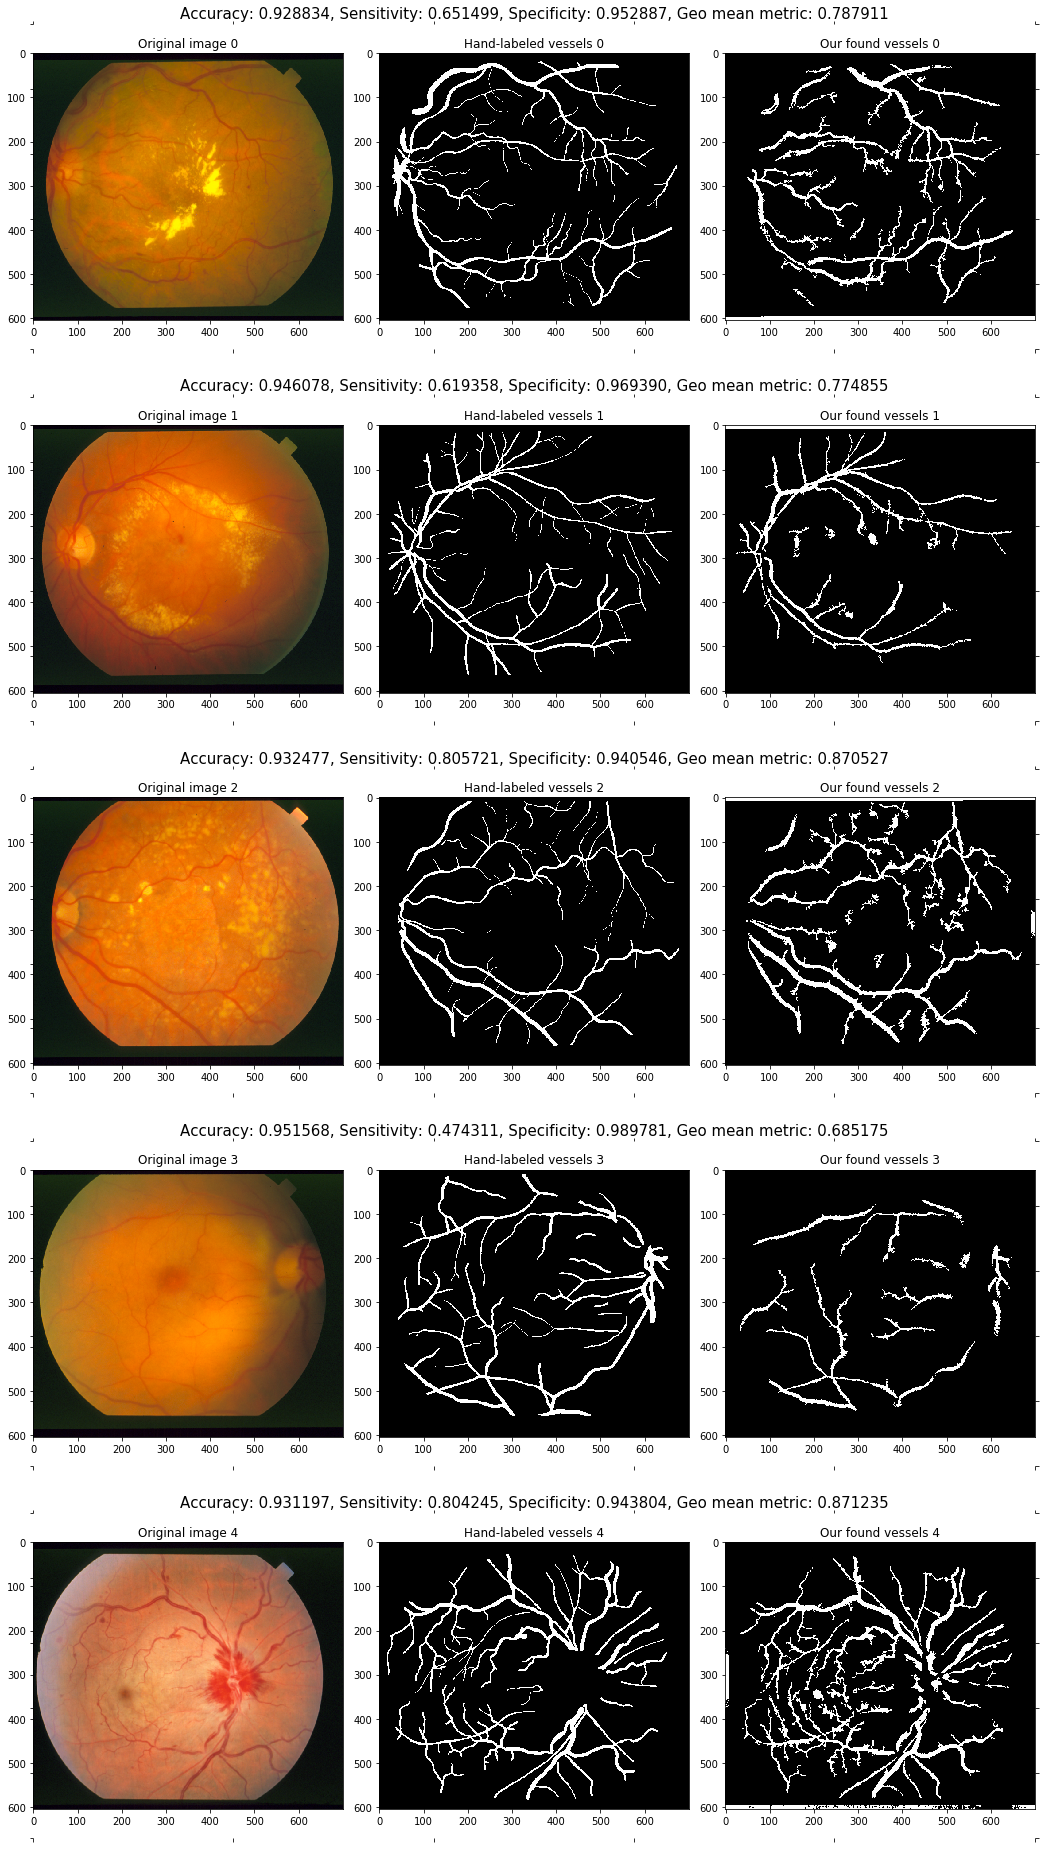
\includegraphics[scale=0.4]{res/oko-1.png}
	\caption{Wyniki uzyskane przy użyciu metod klasycznego przetwarzania obrazu}
	\label{fig:demo}
\end{figure}

\begin{figure}[h]
    \centering
	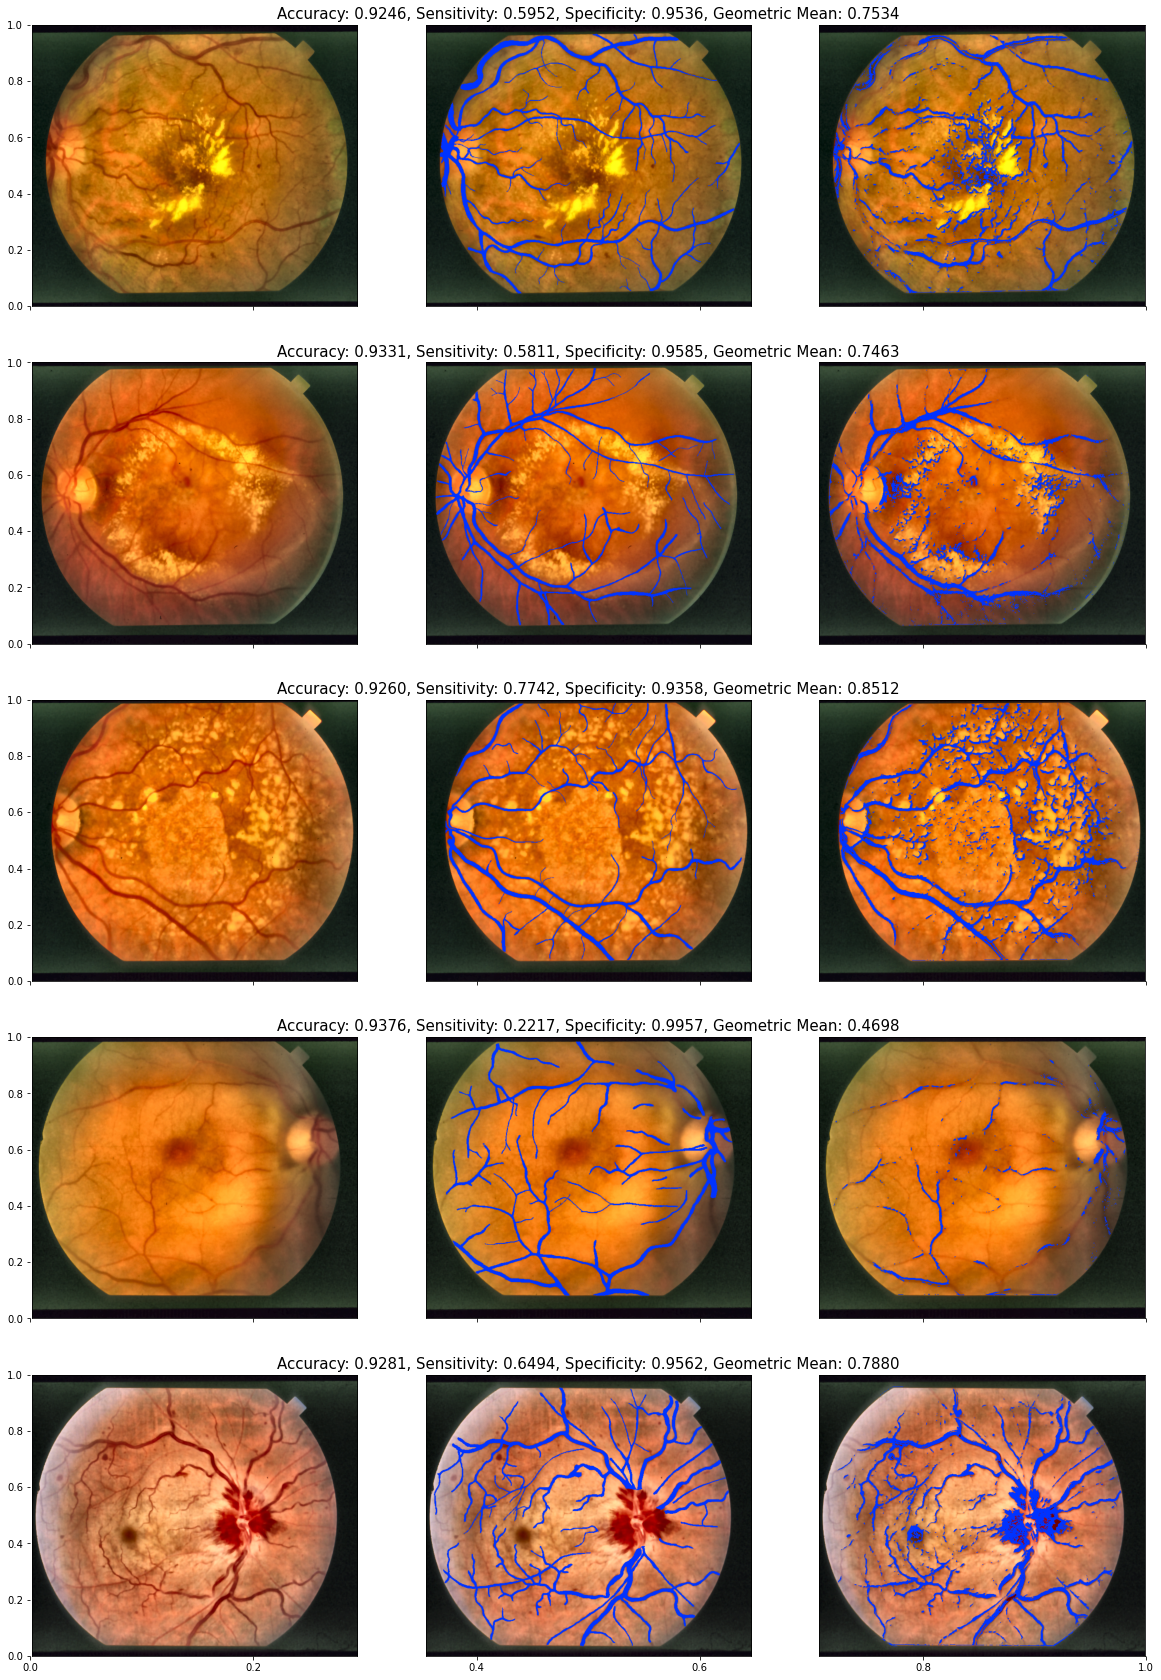
\includegraphics[scale=0.4]{res/oko-2.png}
	\caption{Wyniki uzyskane przy użyciu metod uczenia maszynowego}
	\label{fig:demo}
\end{figure}

\end{document}
